\documentclass[xcolor=dvipsnames]{beamer}
\usepackage[utf8]{inputenc}
\usepackage{times}
\usepackage[T1]{fontenc}
\usepackage{tikz}
\usepackage{pifont}
\usepackage{eurosym}

%% Hacer transparentes las partes ocultas (de otra forma se ocultan totalmente)
\setbeamercovered{transparent}

% Elegir el tema
%\usetheme{JuanLesPins}
%\useinnertheme{rounded}
\useinnertheme{circles}
\setbeamertemplate{blocks}[rounded]

% Poner los colores "lambda"
\DefineNamedColor{named}{ColorLambda}{named}{orange}
\usecolortheme[named={ColorLambda}]{structure}
\definecolor{grisnormal}{RGB}{170,170,170}
\definecolor{verdealerta}{RGB}{86,145,0}

% Otros colores
\setbeamercolor{top heading}{fg=black!30}
\setbeamercolor{section in head/foot}{fg=orange}
\setbeamercolor{subsection in head/foot}{fg=orange!50}
\setbeamercolor{item projected}{fg=black}
\setbeamercolor{description item}{fg=ColorLambda!50!black}
\setbeamercolor{alerted text}{fg=green!50!black}
\setbeamercolor{example text}{fg=ColorLambda!60!red!50!black}

 \setbeamercolor{block title}{use=structure,fg=white,bg=ColorLambda}
 \setbeamercolor{block title alerted}{use=alerted text,fg=white,bg=verdealerta}
 \setbeamercolor{block title example}{use=example text,fg=white,bg=grisnormal}
% 
 \setbeamercolor{block body}{parent=normal text,use=block title,bg=}
 \setbeamercolor{block body alerted}{parent=normal text,use=block title alerted,bg=}
 \setbeamercolor{block body example}{parent=normal text,use=block title example,bg=}


% Logo LambdaStream
\pgfdeclareimage[height=0.75cm]{LogoLambda}{LogoLambda}
%\pgfdeclareimage[height=1cm,width=12cm]{ovalo}{ovalo}
%\pgfdeclareimage[height=0.3cm]{separador}{separador}
% Encabezados y pies
\setbeamertemplate{headline}
{
%\vskip0.3cm
{\usebeamercolor[fg]{top heading} \hspace{0.5cm} \insertshortinstitute \hfill \insertshorttitle} \hspace{0.5cm}
\vspace{0.09cm}
{\usebeamercolor[fg]{top heading} \hrule}
\vspace{0.2cm}
\begin{tiny}{\usebeamercolor[fg]{section in head/foot} \hspace{0.5cm}{\textbf \insertsection}}\hfill %\begin{tiny}{\usebeamercolor[fg]{subsection in head/foot}\insertsubsectionnavigationhorizontal{0.2\paperwidth}{}{}}\end{tiny} 
{\usebeamercolor[fg]{subsection in head/foot}\insertsubsection} \hspace{0.5cm} \end{tiny}
\vskip-1cm
}

\setbeamertemplate{footline}{}


% 
% 
\setbeamertemplate{frametitle}
{
\leftskip=-20pt
%\vskip1cm
\vspace{1.2cm}
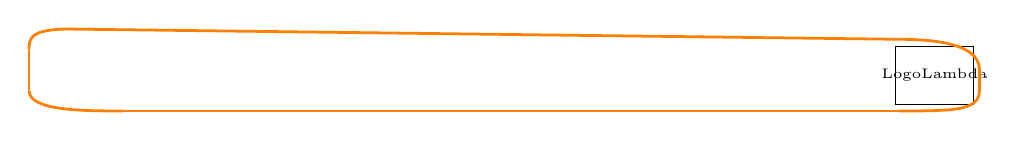
\begin{tikzpicture}
%\draw (0,0) node[anchor=west]{\pgfuseimage{ovalo}};
\draw[color=orange](0.4,0.1) node[anchor=west]{\textbf{\begin{footnotesize}\insertframetitle\end{footnotesize}}};
\draw[color=gray](0.6,-0.3) node[anchor=west]{\textbf{\begin{scriptsize}\insertframesubtitle\end{scriptsize}}};
\draw (11.5,-0.2) node{\pgfuseimage{LogoLambda}};
\begin{scope}[xscale=0.17, yscale=0.13, yshift=-5cm]
\draw[line width=1pt, color=orange] (3,8) .. controls (0,8) and (0,7) .. (0,6);
\draw[line width=1pt, color=orange] (0,6) .. controls (0,6) and (0,2) .. (0,2);
\draw[line width=1pt, color=orange] (0,2) .. controls (0,0) and (4,0) .. (7,0);
\draw[line width=1pt, 	color=orange] (7,0) .. controls (7,0) and (60,0) .. (65,0);
\draw[line width=1pt, color=orange] (65,0) .. controls (69,0) and (71,0) .. (71,2);
\draw[line width=1pt, color=orange] (71,2) .. controls (71,2) and (71,4) .. (71,4);
\draw[line width=1pt, color=orange] (71,4) .. controls (71,6) and (69,7) .. (65,7);
\draw[line width=1pt, color=orange] (65,7) .. controls (65,7) and (3,8) .. (3,8);
\end{scope}
\end{tikzpicture}

}


%% TODO:
%% * Put the sign of Change Ahead

%--------------------------------------------------------------------------------
% Style
%--------------------------------------------------------------------------------
% Libraries
\usetikzlibrary{shapes.symbols}

% Some generalities
\usetheme{default}
\useinnertheme{circles}
\useoutertheme{infolines}
\usecolortheme{crane}
\logo{
\includegraphics[height=1.5cm]{LogoLambda.pdf}}

% Fine-grain control over each section

\setbeamertemplate{headline}{}
\setbeamertemplate{navigation symbols}{}

\setbeamertemplate{footline}{%
  \leavevmode%
  \hbox{%
  \begin{beamercolorbox}[wd=.333333\paperwidth,ht=2.25ex,dp=1ex,center]{author in head/foot}%
    \usebeamerfont{author in head/foot}\insertshortauthor~~(\insertshortdate)
  \end{beamercolorbox}%
  \begin{beamercolorbox}[wd=.333333\paperwidth,ht=2.25ex,dp=1ex,center]{title in head/foot}%
    \usebeamerfont{title in head/foot}\insertshorttitle
  \end{beamercolorbox}%
  \begin{beamercolorbox}[wd=.333333\paperwidth,ht=2.25ex,dp=1ex,center]{date in head/foot}%
    \usebeamerfont{date in head/foot}w~w~w~.~l~a~m~b~d~a~s~t~r~e~a~m~.~c~o~m%
  \end{beamercolorbox}}%
  \vskip0pt%
}

%--------------------------------------------------------------------------------
% Title, authors, etc
%--------------------------------------------------------------------------------

%--------------------------------------------------------------------------------
% Headers
%--------------------------------------------------------------------------------
\title[]{Testing What Should Work, Not What Shouldn't Fail}

\author[Samuel Rivas]{Samuel Rivas}

\institute[LambdaStream]{LambdaStream S.L.\\ <samuel.rivas@lambdastream.com>\\%
  \vspace{1cm}
\includegraphics[width=.30\textwidth]{Logo-ProTest-pos-web.jpg}}

\date[EUC 2010]{EUC'2010 Stockholm}
\subject{Testing}

% TOC before each subsection
% \AtBeginSubsection[]
% {
%   \begin{frame}<beamer>
%     \frametitle{Index}
%     \tableofcontents[currentsection,currentsubsection]
%   \end{frame}
% }

\begin{document}

%--------------------------------------------------------------------------------
% Drawing options and styles
%--------------------------------------------------------------------------------

\usepgflibrary{arrows}
\usetikzlibrary{calc}
\tikzset{every picture/.style=thick, >=stealth}
\tikzset{image/.style={draw, inner sep=0pt, line width=3pt}}
%\tikzset{help lines/.style={blue!50,very thin}}

%--------------------------------------------------------------------------------
% Slides
%--------------------------------------------------------------------------------

\begin{frame}
  \titlepage
\end{frame}

\begin{frame}
  \frametitle{Schedule}

  Today, we have two testing stories for you:

  \begin{itemize}
  \item \textbf{``Testing''} a classical story (with sad ending)
  \item \textbf{``Testing Reloaded''} A Sci-fi remake (with property technology)
  \item \textbf{Behind the Scenes}
  \end{itemize}
\end{frame}

%% TODO: put calligraphy font
\begin{frame}
  \begin{center}
    {\huge Testing}\\
    \vspace{1cm}
    A Classical Story
  \end{center}
\end{frame}

%% TODO: Stress the variable
\begin{frame}[fragile]
  \frametitle{Template Library}

  \begin{block}{Specification}%
\begin{verbatim}
template:apply(
  "@lang@ rulez!", [{"lang", "Erlang"}]) ->

"Erlang rulez!"
\end{verbatim}
  \end{block}
\end{frame}

\begin{frame}[fragile]
  \frametitle{The Test Suite}

\begin{verbatim}
?assertEqual(
   "Erlang rulez!", template:apply(
   "@lang@ rulez!",[{"lang","Erlang"}])

?assertEqual(
   "C sux!", template:apply(
   "@lang@ @what@!",[{"lang","C"},{"what","sux"}])

?assertEqual("Hello", template:apply("Hello",[]))

?assertEqual("", template:apply("",[]))
\end{verbatim}
\end{frame}

%% TODO: Write an arrow pointing to €€€
\begin{frame}
  \frametitle{The Process}
  \begin{center}
    \begin{columns}
      \column{0.4\textwidth}
      \begin{enumerate}
      \item Implement the library
      \item Test it
      \item Fix it
      \item<+-> Test it...
      \item<+-> Fix it again
      \item<.-> Test it
      \item<.-> Ship it
      \end{enumerate}
      \column{0.3\textwidth}
      \onslide<+->{%
        {\huge \textbf{\euro\euro\euro} !!}
      }
    \end{columns}
  \end{center}
\end{frame}

%% TODO: stress the ats
\begin{frame}[fragile]
  \frametitle{Feature Request}

  \begin{block}{Specification}%
\begin{verbatim}
template:apply(
  "samuel.rivas@@lambdastream.com", []) ->

"samuel.rivas@lambdastream.com"
\end{verbatim}
  \end{block}
\end{frame}

\begin{frame}[fragile]
  \frametitle{New Test Cases}

\begin{verbatim}
?assertEqual("@",template:apply("@@",[]))

?assertEqual(
  "samuel.rivas@lambdastream.com",
  template:apply(
    "samuel.rivas@@lambdastream.com",[])
\end{verbatim}
\end{frame}

\begin{frame}
  \frametitle{The Change Process}
  \begin{enumerate}
  \item Implement the library
  \item Test it
  \item Fix it
  \item Ship it
  \end{enumerate}
\end{frame}

\begin{frame}
  \frametitle{What the Customer Got}
  
\includegraphics[width=\textwidth]{images/nuclear}
\end{frame}

\begin{frame}[fragile]
  \frametitle{The Failure}

\begin{block}<+->{Production Code}
\texttt{template:apply(}\\
\texttt{~~"\alert<3>{\alert<2>{@name@}@@\alert<2>{@domain@}}",}\\
\texttt{~~[\{"\alert<2>{name}",   "samuel.rivas"    \},}\\
\texttt{~~~\{"\alert<2>{domain}", "lambdastream.com"\}]).}
\end{block}

\begin{alertblock}<1->{Production Error}
\texttt{exception: \{variable\_not\_found,"\alert<3>{name@@domain}"\}}
\end{alertblock}
\end{frame}

%% TODO: Find a picture
\begin{frame}
  \begin{center}
    {\huge Testing What Should't Fail}\\
    \vspace{1cm}
    And you though the computer would generalise ...
  \end{center}
\end{frame}

\begin{frame}[fragile]
  \frametitle{This Shouldn't Fail}

\begin{verbatim}
?assertEqual(
   "Erlang rulez!", template:apply(
   "@lang@ rulez!",[{"lang","Erlang"}])

?assertEqual("@",template:apply("@@",[]))
\end{verbatim}
\end{frame}

\begin{frame}[fragile]
  \frametitle{Missing Case}
\begin{verbatim}
?assertEqual(
  "foobar", template:apply(
  "@one@@two@",[{"one","foo"},{"two", "bar"}])
\end{verbatim}
\end{frame}

\begin{frame}[plain]
  
\includegraphics[width=\textwidth]{images/matrix}
\end{frame}

\begin{frame}[fragile]
  \frametitle{Template Library}

  \begin{block}{Specification}%
\begin{verbatim}
template:apply(
  "@lang@ rulez!", [{"lang", "Erlang"}]) ->

"Erlang rulez!"
\end{verbatim}
  \end{block}
\end{frame}

\begin{frame}[fragile]
  \frametitle{The (Rough) Property}

  \begin{center}
    \textit{ For all template T, list of variables X, and list of
      substitutions X', apply(T, X) must yield T with X values
      switched to X'}
  \end{center}

  \begin{block}<2->{Erlang Implementation}
\begin{verbatim}
?FORALL(T, template(),
  template:apply(to_string(T), to_subs(T)) ==
  to_result(T)).
\end{verbatim}
  \end{block}
\end{frame}

\begin{frame}[fragile]
  \frametitle{Change!}

  \begin{center}
    \textit{ For all template T, list of variables X, and list of
      substitutions X', apply(T, X) must yield T with X values
      switched to X' \alert{and all escaped at symbols changed to at
        symbols}}
  \end{center}

  \begin{block}{Erlang Implementation}
\verb+?FORALL(T,+\alert{\texttt{template(),}}
\begin{verbatim}
  template:apply(to_string(T), to_subs(T)) ==
  to_result(T)).
\end{verbatim}
  \end{block}
\end{frame}

\begin{frame}[fragile]
  \frametitle{The Counterexample}
  \framesubtitle{The Change isn't Implemented Yet}

\begin{verbatim}
prop_template: ..Failed! After 12 tests.
Shrinking.(1 times)
[escaped_at]
prop_template: Failed! After 1 tests.
[escaped_at]
\end{verbatim}
  {\color{red}
\begin{verbatim}
Template: "@@"
Substs  : []
Expected: "@"
Got     : []
\end{verbatim}
}
\end{frame}

\begin{frame}[fragile]
  \frametitle{Another Counterexample}
  \framesubtitle{Hunting the Bug!}

\begin{verbatim}
prop_template: ..Failed! After 16 tests.
Shrinking....(4 times)
[{var," ",[]},{var," ",[]}]
\end{verbatim}
  {\color{red}
\begin{verbatim}
Template: "@ @@ @"
Substs  : [{" ", ""}]
Expected: ""
Got     : {error, {variable_not_found," @ "}}
\end{verbatim}
}
\end{frame}

%% TODO: Look for an image "under the hood"
\begin{frame}
  \begin{center}
    {\huge Testing What Should Always Work}\\
    \vspace{1cm}

    \textit{ For all template T, list of variables X, and list of
      substitutions X', apply(T, X) must yield T with X values
      switched to X' and all escaped at symbols changed to at symbols}
  \end{center}
\end{frame}

%% TODO: Look for an image "under the hood"
\begin{frame}
  \begin{center}
    {\huge Behind the Scenes}\\
    \vspace{1cm}
    Looking under the hood
  \end{center}
\end{frame}

\begin{frame}[fragile]
  \frametitle{Generating Templates?}

  \begin{center}
    \begin{tikzpicture}
      % \draw[help lines](-6,-1) grid (6,7);

      % Bounding box
      \path (-6,-1) rectangle (6,7);

      \draw (-4,5) node (templ){template()};
      \draw (0,5) node (subst){subst()};
      \draw (-4,2) node (template) {"Hi @name@"};
      \draw (0,2) node (subs) {[\{"name","Samuel"\}]};
      \draw (4,2) node (result) {\alert{??}};

      \draw (0,0 -| template.west) node (funct)[right] {apply(};

      \draw (funct.east) node(arg1)[right] {"Hi @name@",};
      \draw (arg1.east) node(arg2)[right] {[\{"name","Samuel"\}]};
      \draw (arg2.east) node(paren)[right] {)};

      \draw [->] (template) -- (arg1);
      \draw [->] (subs) -- (arg2);
      \draw [->] (templ) -- (template);
      \draw [->] (subst) -- (subs);
      \draw [<->,red] (paren) -| (result) node [midway,left,pos=0.75] {==};
    \end{tikzpicture}
  \end{center}
\end{frame}

\begin{frame}[fragile]
  \frametitle{Symbolic Templates}

  \begin{center}
    \begin{tikzpicture}
      % \draw[help lines](-6,-1) grid (6,7);

      % Bounding box
      \path (-6,-1) rectangle (6,7);

      \draw (0,5) node (symbol){template()};

      \draw (-4,2) node (template) {"Hi @name@"};
      \draw (0,2) node (subs) {[\{"name","Samuel"\}]};
      \draw (4,2) node (result) {"Hi Samuel"};

      \draw (0,0 -| template.west) node (funct)[right] {apply(};

      \draw (funct.east) node(arg1)[right] {"Hi @name@",};
      \draw (arg1.east) node(arg2)[right] {[\{"name","Samuel"\}]};
      \draw (arg2.east) node(paren)[right] {)};

      \draw [->] (symbol) -- (template) node [midway,above,sloped] {to\_strting};
      \draw [->] (symbol) -- (subs) node [midway,above,sloped] {to\_subs};
      \draw [->] (symbol) -- (result) node [midway,above,sloped] {to\_result};
      \draw [->] (template) -- (arg1);
      \draw [->] (subs) -- (arg2);
      \draw [<->,red] (paren) -| (result) node [midway,left,pos=0.75] {==};
    \end{tikzpicture}
  \end{center}
\end{frame}

\begin{frame}
  \frametitle{An Outline of the Symbolic Template Generator}

  \begin{description}[\textbf{template()} ->]
  \item[\textbf{template()} ->] \texttt{list(elements([text(),var()])).}
  \item[\textbf{text()} ->] \texttt{\{text,string()\}.}
  \item[\textbf{var()} ->] \texttt{\{var,string(),string()\}.}
  \end{description}
\end{frame}

\begin{frame}[fragile]
  \frametitle{Symbolic Templates}

  \begin{center}
    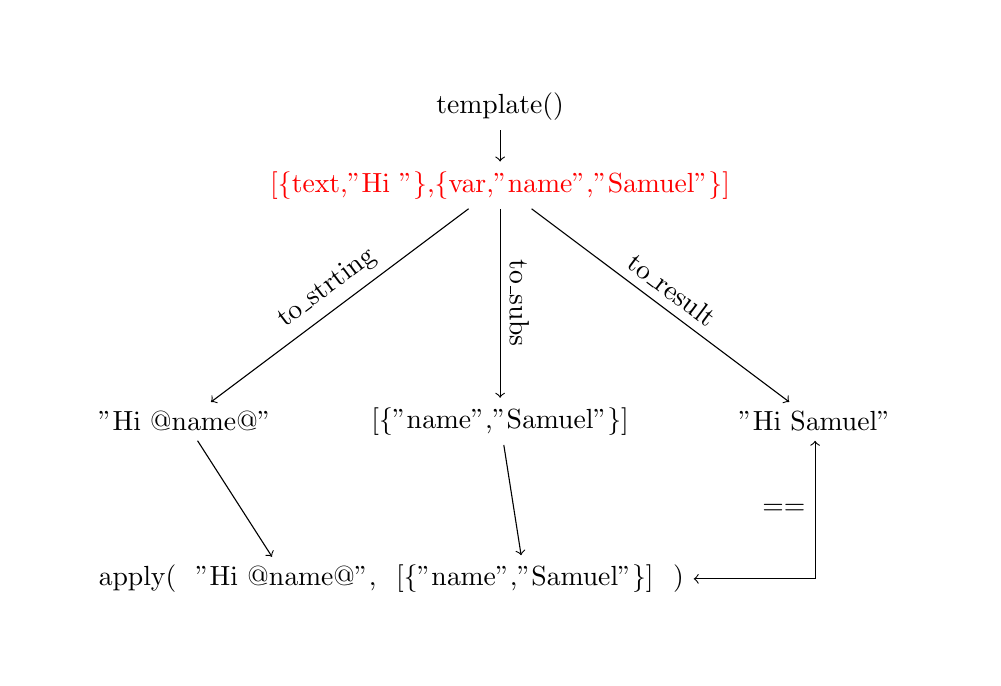
\begin{tikzpicture}
      % \draw[help lines](-6,-1) grid (6,7);

      % Bounding box
      \path (-6,-1) rectangle (6,7);

      \draw (0,6) node (gen){template()};
      \draw[red] (0,5) node (symbol){[\{text,"Hi "\},\{var,"name","Samuel"\}]};
      \draw (-4,2) node (template) {"Hi @name@"};
      \draw (0,2) node (subs) {[\{"name","Samuel"\}]};
      \draw (4,2) node (result) {"Hi Samuel"};

      \draw (0,0 -| template.west) node (funct)[right] {apply(};

      \draw (funct.east) node(arg1)[right] {"Hi @name@",};
      \draw (arg1.east) node(arg2)[right] {[\{"name","Samuel"\}]};
      \draw (arg2.east) node(paren)[right] {)};

      \draw [->] (gen) -- (symbol);
      \draw [->] (symbol) -- (template) node [midway,above,sloped] {to\_strting};
      \draw [->] (symbol) -- (subs) node [midway,above,sloped] {to\_subs};
      \draw [->] (symbol) -- (result) node [midway,above,sloped] {to\_result};
      \draw [->] (template) -- (arg1);
      \draw [->] (subs) -- (arg2);
      \draw [<->] (paren) -| (result) node [midway,left,pos=0.75] {==};
    \end{tikzpicture}
  \end{center}
\end{frame}

\begin{frame}[fragile]
  \frametitle{The Property}

  {\color{red}
\begin{verbatim}
?FORALL(T, template(),
  template:apply(to_string(T), to_subs(T)) ==
  to_result(T)).
\end{verbatim}
  }

  \vspace{0.5cm}
  \begin{center}
    \textit{\footnotesize For all template T, list of variables X, and
      list of substitutions X', apply(T, X) must yield T with X values
      switched to X'}
  \end{center}
\end{frame}

\begin{frame}[fragile]
  \frametitle{Templates 2.0 (With Escaped Ats)}

  \begin{center}
    \begin{tikzpicture}
%      \draw[help lines](-6,0) grid (6,6);

      % Bounding box
      \path (-6,-1) rectangle (6,7);

      \draw (0,5) node (symbol) {[\alert{escaped\_at}]};

      \draw (0,6) node (gen){template()};
      \draw (-4,2) node (template) {"\alert{@@}"};
      \draw (0,2) node (subs) {[]};
      \draw (4,2) node (result) {"\alert{@}"};
      \draw (0,0 -| template.west) node (funct)[right] {apply(};
      \draw (funct.east) node(arg1)[right] {"@@",};
      \draw (arg1.east) node(arg2)[right] {[]};
      \draw (arg2.east) node(paren)[right] {)};

      \draw [->] (gen) -- (symbol);
      \draw [->] (symbol) -- (template) node [midway,above,sloped] {to\_string};
      \draw [->] (symbol) -- (result) node [midway,above,sloped] {to\_result};
      \draw [->] (symbol) -- (subs) node [midway,above,sloped] {to\_subs};
      \draw [->] (template) -- (arg1);
      \draw [->] (subs) -- (arg2);
      \draw [<->] (paren) -| (result) node [midway,above,pos=0.25] {==};
    \end{tikzpicture}
  \end{center}
\end{frame}

\begin{frame}[fragile]
  \frametitle{The Counterexample Hero}

  \begin{center}
    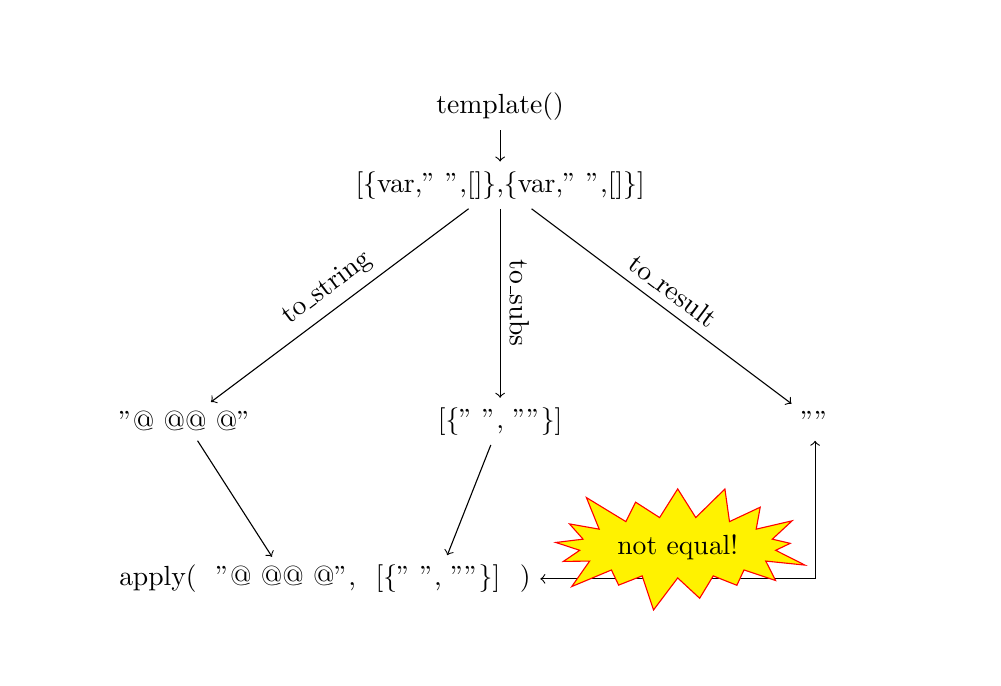
\begin{tikzpicture}
%      \draw[help lines](-6,0) grid (6,6);

      % Bounding box
      \path (-6,-1) rectangle (6,7);

      \draw (0,5) node (symbol) {[\{var," ",[]\},\{var," ",[]\}]};


      \draw (0,6) node (gen){template()};
      \draw (-4,2) node (template) {"@ \alert{@@} @"};
      \draw (0,2) node (subs) {[\{" ", ""\}]};
      \draw (4,2) node (result) {""};
      \draw (0,0 -| template.west) node (funct)[right] {apply(};
      \draw (funct.east) node(arg1)[right] {"@ @@ @",};
      \draw (arg1.east) node(arg2)[right] {[\{" ", ""\}]};
      \draw (arg2.east) node(paren)[right] {)};

      \draw [->] (gen) -- (symbol);
      \draw [->] (symbol) -- (template) node [midway,above,sloped] {to\_string};
      \draw [->] (symbol) -- (result) node [midway,above,sloped] {to\_result};
      \draw [->] (symbol) -- (subs) node [midway,above,sloped] {to\_subs};
      \draw [->] (template) -- (arg1);
      \draw [->] (subs) -- (arg2);
      \draw [<->] (paren) -| (result) node [starburst,draw,fill=yellow,
      draw=red,midway,above,pos=0.25] {not equal!};
    \end{tikzpicture}
  \end{center}
\end{frame}

\begin{frame}
  \begin{center}
    {\huge Conclusions}\\
  \end{center}
\end{frame}

\begin{frame}
  \frametitle{Conclusions}
  \begin{itemize}
  \item Test cases test \textit{what shouldn't fail}
  \item Properties test \textit{what should always work}
  \item Properties resist better in changing conditions
  \end{itemize}
\end{frame}

%% TODO: Think of the image of Change Ahead --> properties!

\begin{frame}
  \frametitle{Thanks For Your Attention!}
  \begin{center}
    \huge{Questions?}\\
    \vspace{1cm}
    \normalsize
    Code available in Github: \color{blue}{http://github.com/lambdastream/tdd\_template}
  \end{center}
\end{frame}

\begin{frame}
  \titlepage
\end{frame}
\end{document}

\end{document}

\begin{frame}[fragile]
  \frametitle{The Result of Our TDD Process}

  \begin{block}{Template library}
\begin{verbatim}
string(String, Subs) ->
    apply_subs(parse(tokens(String)), Subs).
\end{verbatim}
  \end{block}


  \begin{block}{Tests}%
\begin{verbatim}
?assertEqual(
   "hello Samuel",
   lstd_template:string(
     "hello @name@", [{"name", "Samuel"}]).
\end{verbatim}
  \end{block}
\end{frame}

\begin{frame}
  \frametitle{A Year Later}

  \begin{itemize}
  \item A good paying customer wants to use @ symbols in static text
  \item Write a new test:\\
    \texttt{"@" == lstd\_template:string("@@", []).}
  \item Fix the code, run the tests. They pass \ding{52}
  \item Ship the code
  \end{itemize}
\end{frame}

\begin{frame}[fragile]
  \frametitle{Were Our Tests Strong Enough?}

\begin{block}<+->{Production Code}
\begin{verbatim}
lstd_template:string(
  "@name@@@@domain@",

  [{"name",   "samuel.rivas"    },
   {"domain", "lambdastream.com"}]).
\end{verbatim}
\end{block}

\begin{alertblock}<+>{Production Error}
\begin{verbatim}
exception: {variable_not_found,"name@@domain"}
\end{verbatim}
\end{alertblock}
\end{frame}

\begin{frame}
  \frametitle{Why?}

  \begin{itemize}
  \item It's a corner case that our tests were not covering
  \item Probably, the bug was not in the original implementation
  \item The last developer only wrote tests to check the new behaviour
  \item \alert{The tests were not preserving the behaviour, they were just
      testing that the initial implementation was ok}
  \end{itemize}
\end{frame}

\begin{frame}[fragile]
  \frametitle{More Conservative Testing}

    \begin{block}{Add more tests}
\begin{verbatim}
?assertEqual(  % We had a bug with this!
   "Samuel@udc.es",
   lstd_template:string(
     "@name@@@udc.es", [{"name", "Samuel"}])).

?assertEqual(  % What if the result is ""?
   "",lstd_template:string("@var@",[{"var", ""}])).

?assertEqual(  % Could \n become special?
   "Text\nwith lines",
   lstd_template:string(
     "@var@\nwith lines", [{"var", "Text"}])).
\end{verbatim}
    \end{block}
\end{frame}

\begin{frame}
  \frametitle{Too much code!}
  \begin{itemize}
  \item Even for simple modules, it is difficult to cover all cases
  \item Increasing logic coverage makes tests more difficult to maintain
    \begin{itemize}
    \item We'll start travelling heavy
    \end{itemize}
  \item How to foresee what can be a corner case in the future?
  \end{itemize}
\end{frame}

\begin{frame}[fragile]
  \frametitle{Property Based Testing}

  \begin{block}{QuickCheck}
    \begin{itemize}
    \item Describe properties about the system
    \item Let the computer generate the tests
    \end{itemize}
  \end{block}
  \begin{exampleblock}{reverse(L1 ++ L2) == reverse(L2) ++ reverse(L1)}
\scriptsize
\begin{verbatim}
reverse([] ++ [1]) == reverse([1]) ++ lists:reverse([])
reverse([] ++ [-1]) == reverse([-1]) ++ lists:reverse([])
reverse([-2] ++ [2]) == reverse([2]) ++ lists:reverse([-2])
reverse([3,4] ++ []) == reverse([]) ++ lists:reverse([3,4])
reverse([-4,3] ++ []) == reverse([]) ++ lists:reverse([-4,3])
reverse([] ++ [-2,1]) == reverse([-2,1]) ++ lists:reverse([])
reverse([7] ++ [7,-4,-8]) == reverse([7,-4,-8]) ++ lists:reverse([7])
reverse([-2] ++ [-6,-4,0]) == reverse([-6,-4,0]) ++ lists:reverse([-2])
...
\end{verbatim}
  \end{exampleblock}
\end{frame}

\begin{frame}[fragile]
  \frametitle{First Property}

  \begin{block}{Rough Specification}
    A template is a string with variables that can be substituted
  \end{block}


  \begin{block}{Forall S, lstd\_template:string(S, []) == S}
\begin{verbatim}
prop_string_empty_list() ->
    ?FORALL(
       S, q_gen:string(),
       S =:= lstd_template:string(S, [])).
\end{verbatim}
  \end{block}

    \begin{exampleblock}{Implementation}
\begin{verbatim}
string(S, []) -> S.
\end{verbatim}
    \end{exampleblock}

\end{frame}

\begin{frame}
  \frametitle{Next Step?}

  \begin{itemize}
  \item Define the substitution process
  \item Write a new property about that and work to pass all generated tests
  \item If writing such a property is difficult, write lower level properties
  \end{itemize}
\end{frame}

\begin{frame}[fragile]
  \frametitle{Symbolic Representations}

  \begin{itemize}
  \item Design a symbolic representation of a template
  \item Write a generator to create those representations
  \item Write rules to create inputs and outputs from symbolic template
  \item Write properties reasoning about the representation, using generated
    inputs and expected outputs
  \end{itemize}

  \begin{block}{Symbolic Templates}
\begin{verbatim}
template()=[var()|text()]
var()={var,string(),string()}
text()={text,string()}
\end{verbatim}
  \end{block}
\end{frame}

\begin{frame}[fragile]
  \frametitle{Symbolic Templates}

  \begin{center}
    \begin{tikzpicture}
%      \draw[help lines](-6,0) grid (6,6);

      % Bounding box
      \path (-6,0) rectangle (6,6);

      \draw<1-> (0,5) node (symbol){[\{text,"Hi "\},\{var,"name","Samuel"\}]};
      \draw<2-> (-4,2) node (template) {"Hi @name@"};
      \draw<3-> (0,1) node (subs) {[\{"name","Samuel"\}]};
      \draw<4-> (4,2) node (result) {"Hi Samuel"};

      \draw<2-> [->] (symbol) -- (template) node [midway,above,sloped] {to\_strting};
      \draw<3-> [->] (symbol) -- (subs) node [midway,above,sloped] {to\_subs};
      \draw<4-> [->] (symbol) -- (result) node [midway,above,sloped] {to\_result};
    \end{tikzpicture}
  \end{center}
\end{frame}

\begin{frame}[fragile]
  \frametitle{The property}
\begin{verbatim}
prop_string() ->
  ?FORALL(T,template(),
    to_result(T)==
      string(to_string(T),to_subs(T))).
\end{verbatim}
\end{frame}

\begin{frame}[fragile]
  \frametitle{Symbolic Template Generator}
\begin{verbatim}
template() ->
    eqc_gen:list(eqc_gen:oneof([text(), var()])).

text() ->
    {text, string()}.

var() ->
    {var, string(), string()}.
\end{verbatim}
\end{frame}


\begin{frame}
  \frametitle{Specify the Scanner}

  \begin{itemize}
  \item Trying to write the substitution function from scratch is too hard
  \item We decide to divide the problem in three steps
    \begin{itemize}
    \item Write a scanner
    \item Write a parser
    \item Implement the substitution process
    \end{itemize}
  \end{itemize}
  \begin{block}{Next Steps}
    \begin{itemize}
    \item Define the function to map symbolic templates to tokens
    \item Write a property
    \item Work to pass the generated tests
    \end{itemize}
  \end{block}
\end{frame}

\begin{frame}
  \frametitle{Converter to Scanner Results}
  \begin{center}
    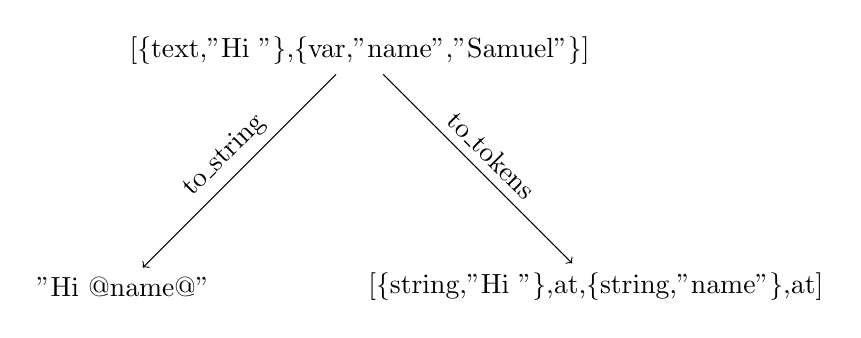
\begin{tikzpicture}
      % \draw[help lines](-6,0) grid (6,6);

      \draw (0,5) node (symbol){[\{text,"Hi "\},\{var,"name","Samuel"\}]};
      \draw (-3,2) node (template) {"Hi @name@"};
      \draw (3,2) node (toks) {[\{string,"Hi "\},at,\{string,"name"\},at]};

      \draw [->] (symbol) -- (template) node [midway,above,sloped] {to\_string};
      \draw [->] (symbol) -- (toks) node [midway,above,sloped] {to\_tokens};
    \end{tikzpicture}
  \end{center}
\end{frame}

\begin{frame}[fragile]
  \frametitle{The Scanner Property}
  \begin{block}{Property}
\begin{verbatim}
prop_tokens() ->
   ?FORALL(T,template(),
      to_tokens(T)==
           lstd_template:tokens(to_string(T))).
\end{verbatim}
  \end{block}
  \begin{center}
    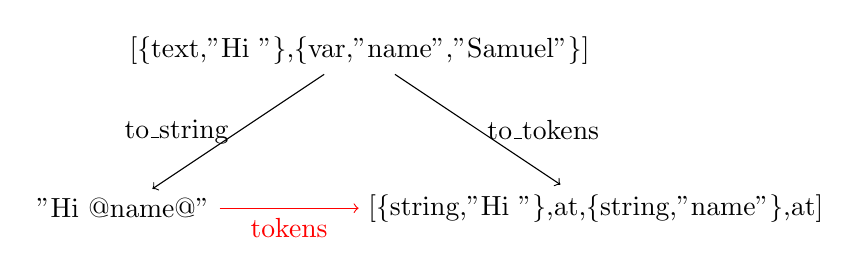
\begin{tikzpicture}
      % \draw[help lines](-6,0) grid (6,6);

      \draw (0,2) node (symbol) {[\{text,"Hi "\},\{var,"name","Samuel"\}]};
      \draw (-3,0) node (input) {"Hi @name@"};
      \draw (3,0) node (tokens) {[\{string,"Hi "\},at,\{string,"name"\},at]};

      \draw[->] (symbol) -- (input) node [midway,left] {to\_string};
      \draw[->] (symbol) -- (tokens) node [midway,right] {to\_tokens};
      \draw[->,red] (input) -- (tokens) node [midway,below] {tokens};
    \end{tikzpicture}
  \end{center}
\end{frame}

\begin{frame}
 \frametitle{Develop the Scanner}

 \begin{itemize}
 \item Previous property will generate failing test cases
 \item We will implement a \texttt{tokens} function hoping to pass them
 \item After we produce the first version of \texttt{tokens} we start fixing
   errors
 \item Typically, the first errors are inconsistencies in the specification
 \end{itemize}
\end{frame}

\begin{frame}
  \frametitle{Inconsistency Example}

  \begin{alertblock}{Tests Fail!}
    \begin{description}[Smaller Counterexample]
    \item<+->[Counterexample] [\{var,"~",""\},\{var,"<0)",""\},\{var,"@b39",""\}]
    \item<+->[Smaller Counterexample] [\{var,"@",""\}]
    \end{description}
  \end{alertblock}

  \begin{center}
    \begin{columns}

      \column{.29\textwidth}
      \begin{block}<+->{Input String} "@@@"
      \end{block}
      \column{.3\textwidth}

      \begin{block}<+->{Expected Output} [at,\{string,"@"\},at]
      \end{block}
      \column{.29\textwidth}

      \begin{alertblock}<+->{Result} [at,at,at]
      \end{alertblock}
    \end{columns}
  \end{center}
  \begin{block}<+->{Solution}
    Avoid @ symbols in generated strings with the generator
    \texttt{valid\_string()}
  \end{block}

\end{frame}

\begin{frame}[fragile]
  \frametitle{Implementing the Parser}

  \begin{block}{Property}
\begin{verbatim}
prop_parse() ->
  ?FORALL(T,template(),
    to_parsed(T)==
      lstd_template:parse(tokens(to_string(T)))).
\end{verbatim}
  \end{block}

  \begin{center}
    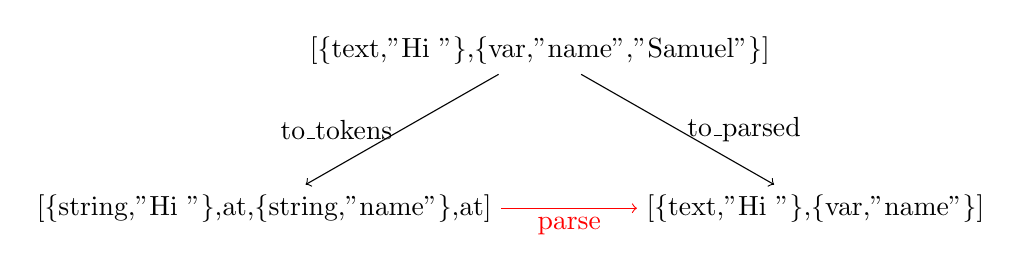
\begin{tikzpicture}
      % \draw[help lines](-6,0) grid (6,6);

      \draw (0,2) node (symbol){[\{text,"Hi "\},\{var,"name","Samuel"\}]};
      \draw (-3.5,0) node (input) {[\{string,"Hi "\},at,\{string,"name"\},at]};
      \draw (3.5,0) node (parsed) {[\{text,"Hi "\},\{var,"name"\}]};

      \draw[->] (symbol) -- (input) node [midway,left] {to\_tokens};
      \draw[->] (symbol) -- (parsed) node [midway,right] {to\_parsed};
      \draw[->,red] (input) -- (parsed) node [midway,below] {parse};
    \end{tikzpicture}
  \end{center}
\end{frame}

\begin{frame}[fragile]
  \frametitle{Parser Ready!}

  \begin{itemize}
  \item Few inconsistencies detected after implemented the parser
    \begin{itemize}
    \item Generators and converters are more stable now
    \end{itemize}
  \item We can reliably parse string templates into a data structure easier to
    handle
  \item We can now implement the substitution process
  \end{itemize}

  \begin{exampleblock}{The parser working}
\begin{verbatim}
> lstd_template:parse("Hi @name@").
[{text,"Hi "},{var,"name"}]
\end{verbatim}
  \end{exampleblock}
\end{frame}

\begin{frame}[fragile]
  \frametitle{Implementing the Substitution Process}

  \begin{block}{Property}
\begin{verbatim}
prop_string() ->
  ?FORALL(T,template(),
    to_result(T)==
      lstd_template:string(
        parse(tokens(to_string(T))),
        to_subs(T))).
\end{verbatim}
  \end{block}

  \begin{center}
    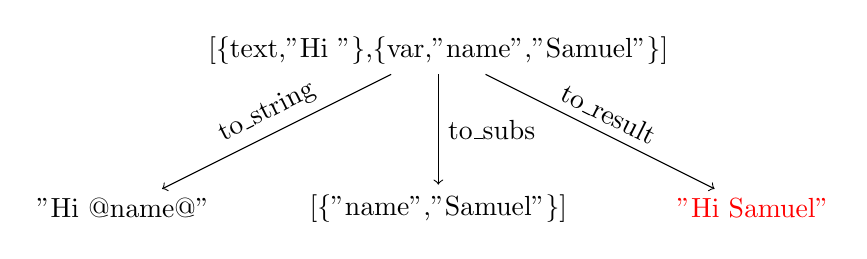
\begin{tikzpicture}
      % \draw[help lines](-6,0) grid (6,6);

      \draw (0,2) node (symbol){[\{text,"Hi "\},\{var,"name","Samuel"\}]};
      \draw (-4,0) node (input) {"Hi @name@"};
      \draw (0,0) node (subs) {[\{"name","Samuel"\}]};
      \draw[red] (4,0) node (result) {"Hi Samuel"};

      \draw [->] (symbol) -- (input) node [midway,above,sloped] {to\_string};
      \draw [->] (symbol) -- (subs) node [midway,right] {to\_subs};
      \draw [->] (symbol) -- (result) node [midway,above,sloped] {to\_result};
    \end{tikzpicture}
  \end{center}
\end{frame}

\begin{frame}
  \frametitle{Implementation Ready!}

  \begin{itemize}
  \item At this point, no more inconsistencies in the properties were found
  \item Once we finished an implementation that passed all generated tests we
    are ready to ship
  \end{itemize}


\end{frame}

\begin{frame}[fragile]
  \frametitle{Introducing Little Changes}

  \begin{itemize}
  \item The first version of the library is in production
  \item But we can't use @ symbols as static text
  \item What if we want to allow escaped @ symbols?
  \end{itemize}
  \begin{block}{Allowing Escaped Ats}
    \texttt{> string("\alert{@@} allowed:@at@",[\{"at","true"\}]).}\\
    \texttt{"\alert{@} allowed:true"}
  \end{block}
\end{frame}

\begin{frame}
  \frametitle{Updating the Properties}

  \begin{itemize}
  \item Our properties already describe the system, specifying three steps:
    scanning, parsing, substituting
  \item Those steps doesn't change
  \item The main logic doesn't change
  \item In this case, we only need updating the symbolic representation
  \end{itemize}
\end{frame}

\begin{frame}[fragile]
  \frametitle{Symbolic Templates With Escaped Ats}

  \begin{center}
    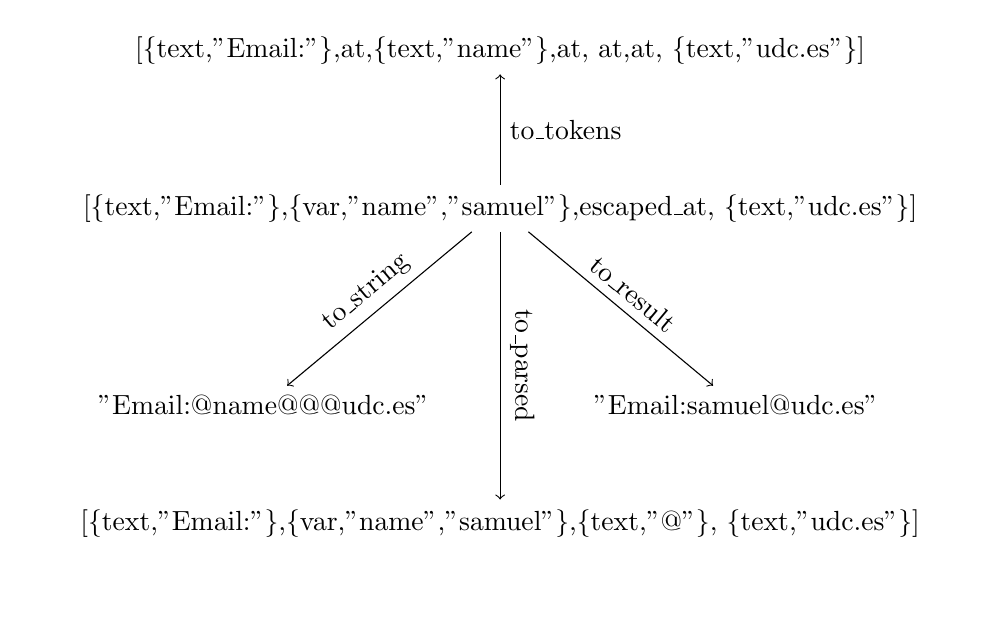
\begin{tikzpicture}
%      \draw[help lines](-6,0) grid (6,6);

      % Bounding box
      \path (-6,0) rectangle (6,6);

      \draw (0,7) node (toks) {[\{text,"Email:"\},at,\{text,"name"\},at,
        \alert{at,at}, \{text,"udc.es"\}]};

      \draw (0,5) node (symbol)
      {[\{text,"Email:"\},\{var,"name","samuel"\},\alert{escaped\_at},
        \{text,"udc.es"\}]};

      \draw (-3,2.5) node (template) {"Email:@name@\alert{@@}udc.es"};
      \draw (3,2.5) node (result) {"Email:samuel\alert{@}udc.es"};

      \draw (0,1) node (parsed)
      {[\{text,"Email:"\},\{var,"name","samuel"\},\alert{\{text,"@"\}},
        \{text,"udc.es"\}]};

      \draw [->] (symbol) -- (template) node [midway,above,sloped] {to\_string};
      \draw [->] (symbol) -- (toks) node [midway,right] {to\_tokens};
      \draw [->] (symbol) -- (result) node [midway,above,sloped] {to\_result};
      \draw [->] (symbol) -- (parsed) node [midway,above,sloped] {to\_parsed};
    \end{tikzpicture}
  \end{center}
\end{frame}

\begin{frame}[fragile]
  \frametitle{Start With the Smallest Counterexample}

  Running the tests reveal that we only broke prop\_parse
  \begin{alertblock}{Counterexample}
\begin{verbatim}
prop_parse: ..Failed! After 12 tests.
[{text,"5"},escaped_at]
Shrinking.(1 times)
[escaped_at]
prop_string: Failed! After 1 tests.
[escaped_at]

Template: "@@"
Substs  : []
Expected: "@"
Got     : []
\end{verbatim}
  \end{alertblock}
\end{frame}

\begin{frame}[fragile]
  \frametitle{Mistaken Implementation}

  \begin{exampleblock}<+->{Too Easy}
\begin{verbatim}
parse([at,at|T],Terminal)->
    [{text,"@"}|parse(T,Terminal)];
parse([at|T],Terminal)->
    parse(T,switch_terminal(Terminal));
\end{verbatim}
  \end{exampleblock}
  \begin{alertblock}<+->{Ouch! prop\_parse doesn't hold for \texttt{"@ @@ @"}}
    \begin{overprint}
      \onslide<.>
\begin{verbatim}
...............Failed! After 16 tests.
[{var,"\r","\""},{var,"\f(d",[]}]
Shrinking....(4 times)
[{var," ",[]},{var," ",[]}]
\end{verbatim}
      \onslide<+>
\texttt{> lstd\_template:parse("@ \alert{@@} @").}\\
\texttt{[\{var," "\},\alert{\{text,"@"\}},\{var," "\}]}
    \end{overprint}
  \end{alertblock}
\end{frame}

\begin{frame}
  \frametitle{Great Coverage!}

  \begin{itemize}
  \item We introduced the corner case in last change
  \item Our previous tests could not anticipate it
  \item But previous tests did find the bug!
  \end{itemize}
  \begin{block}<2>{Why did that work?}
    \begin{itemize}
    \item We haven't changed the properties, just minor details of the
      symbolic representation
    \item All properties must still hold
    \item QuickCheck brute-force coverage
    \end{itemize}
  \end{block}
\end{frame}

\begin{frame}[fragile]
  \frametitle{A Hidden Bug}

  \uncover<2>{Better after shrinking...}

  \begin{block}{This May Happen Now and Then}
    \begin{overprint}
      \onslide<+>
\begin{verbatim}
prop_string: .....Failed! After 48 tests.
[{var,"?%",[]},      {var,"W<ZY","y)8uFE"},
 {text,":5OH\r'"},   {var,"sPtd","` 2"},
 {var,"k","(\eg\v"}, {var,"k","\e4<?bi"}]

Template: "@%@@<ZY@:5OH\r'@sPtd@@k@@k@"
Substs  : [{"%",[]},{"<ZY","y)8uFE"},{"sPtd","` 2"},
           {"k","(\eg\v"},{"k","\e4<?bi"}]
Expected: "y)8uFE:5OH\r'` 2(\eg\v\e4<?bi"
Got     : "y)8uFE:5OH\r'` 2(\eg\v(\eg\v"
\end{verbatim}
      \onslide<+>
\begin{verbatim}
Shrinking.....(5 times)
[{var,"k",[]},{var,"k"," "}]

Template: "@k@@k@"
Substs  : [{"k",[]},{"k"," "}]
Expected: " "
Got     : []
\end{verbatim}
    \end{overprint}
  \end{block}
\end{frame}

\begin{frame}[fragile]
  \frametitle{The Bug}

  \begin{center}
    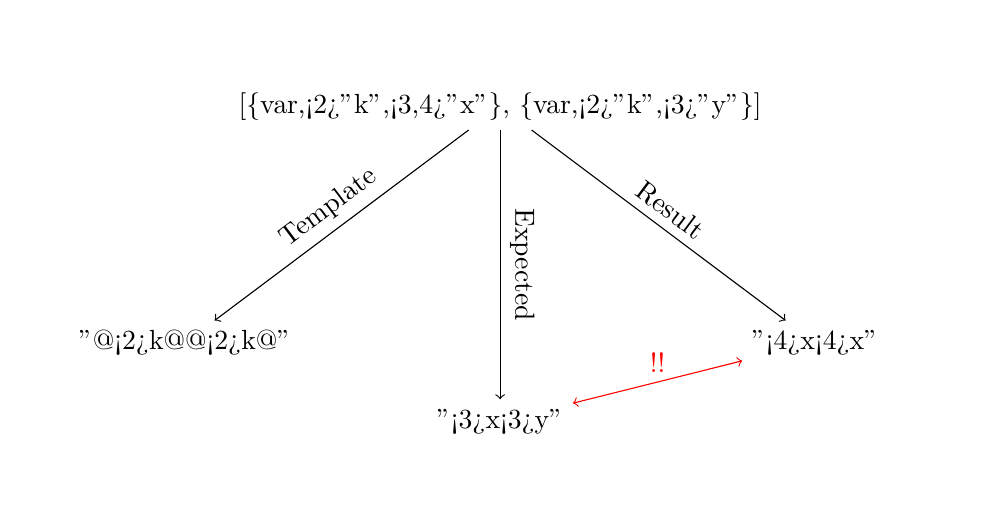
\begin{tikzpicture}
%      \draw[help lines](-6,0) grid (6,6);

      % Bounding box
      \path (-6,0) rectangle (6,6);

      \draw<1-> (0,5) node (symbol) {[\{var,\alert<2>{"k"},\alert<3,4>{"x"}\},
        \{var,\alert<2>{"k"},\alert<3>{"y"}\}]};

      \draw<2-> (-4,2) node (template) {"@\alert<2>{k}@@\alert<2>{k}@"};
      \draw<3-> (0,1) node (expect) {"\alert<3>{x}\alert<3>{y}"};
      \draw<4-> (4,2) node (result) {"\alert<4>{x}\alert<4>{x}"};

      \draw<2-> [->] (symbol) -- (template) node [midway,above,sloped] {Template};
      \draw<3-> [->] (symbol) -- (expect) node [midway,above,sloped] {Expected};
      \draw<4-> [->] (symbol) -- (result) node [midway,above,sloped] {Result};
      \draw<4-> [red,<->] (expect) -- (result) node [midway,above]{!!};
    \end{tikzpicture}
    \uncover<4->{The symbolic representation generated is inconsistent}
  \end{center}
\end{frame}

\begin{frame}[fragile]
  \frametitle{Why The Tests Seldom Hit This Bug?}

  \begin{itemize}
  \item \texttt{valid\_string} generates a random string each time
  \item The odds of generating two variables with the same name are too low
  \end{itemize}

  \begin{block}{The template generator}
\begin{verbatim}
> eqc_gen:sample(lstd_template_eqc:var()).
{var,"\r^H","*AP:"}
{var,"^P.",[]}
{var,"\nkGI",[]}
{var,"A\e(","9\eU~"}
{var,"vBAZ","|/@\tj"}
{var,"x","=Di?n"}
{var,"mmb9:07","sT\n=F1"}
...
\end{verbatim}
  \end{block}
\end{frame}

\begin{frame}
  \frametitle{Test Distribution}
  \begin{itemize}
  \item Good test distribution is essential
  \item Bad test distribution may leave important tests undone
  \item Developers must be aware of this when writing generators
  \item Some intuition is required detect poor test distributions
  \end{itemize}
\end{frame}

\begin{frame}
  \frametitle{PDD Process}

  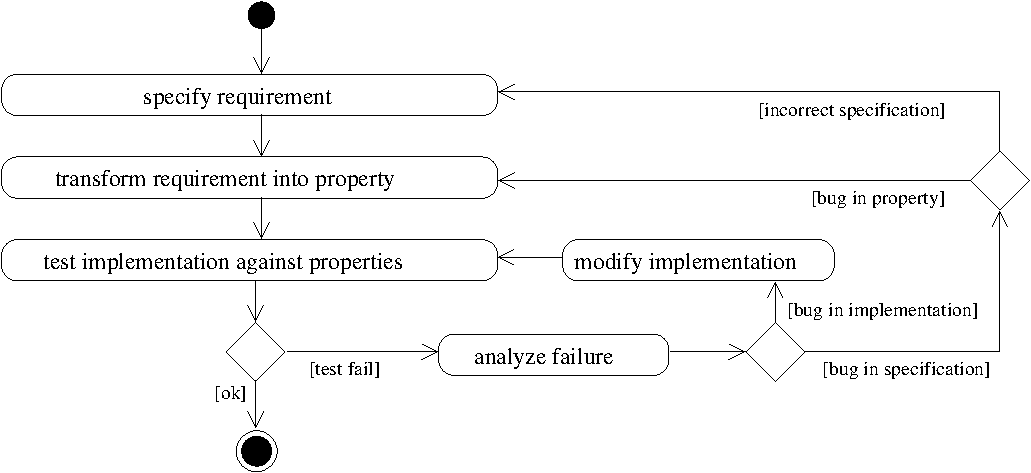
\includegraphics[width=\textwidth]{pdd_process}
\end{frame}

\begin{frame}
  \frametitle{Conclusions}
  \begin{itemize}
  \item Properties are more likely to preserve behaviour across evolutionary
    changes than traditional tests
  \item A good symbolic representation of the system makes property base testing
    easier
  \item Property driven development make resulting code easier to reason about
    using properties
  \item Programmers must watch the statistical distribution of their tests
  \end{itemize}
\end{frame}

\begin{frame}
  \frametitle{Thanks For Your Attention!}
  \begin{center}
    \huge{Questions?}\\
    \vspace{1cm}
    \normalsize
    Code available in Github: \color{blue}{http://github.com/lambdastream/tdd\_template}
  \end{center}
\end{frame}

\begin{frame}
  \titlepage
\end{frame}
\end{document}
